

\partabstractfp{\textbf{进程第1天课程摘要} }
\partabstractrp{}
\partabstractlettrine{}{} % the first word of the abstract

\part{进程课第1天}

\chapter{进程的代码结构}
\section{进程控制块PCB与task\_struct}
进程是一个资源封装的单位,资源指占用的内存,文件系统,信号及处理方法。线程是调度执行的单元。一个进程区别与另一个进程的标记就是资源。linux操作系统是可以做到进程与进程之间的资源隔离。进程的描述就是资源的描述。PCB (PROCESS CONTROL BLOCK) 在不同操作系统中用于描述进程,在Linux的PCB就是用task\_struct来描述。如\ref{linux_pcb}所示,图中列出了主要对应包含的资源种类及作用。
\begin{figure}[H]
 \wdfigbox
  {\caption{fork进程前后内存映射关系}\label{linux_pcb}}
  {
  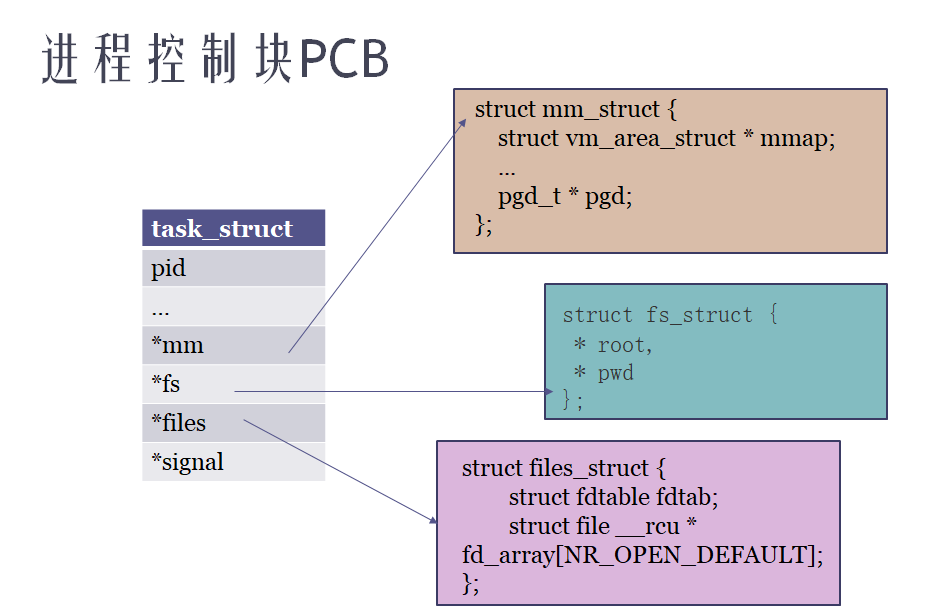
\includegraphics[width=9cm]{./figure/linux_pcb.png}
  \floatfoot{注:第一列为虚拟地址,第二列为物理地址,最后一列对应内存的读写权限 }
  }
\end{figure}
\begin{description}
  \item[\heiti{mm 内存资源:}] 进程的内存
  \item[\heiti{fs 文件系统资源1:}] 根路径和当前路径指针
  \item[\heiti{files 文件系统资源2:}] 进程打开的文件,文件描述符数组
  \item[\heiti{sinal 信号资源:}] 不同进程可以针对同一信号挂不同的处理方法
  \item[\heiti{pid 属性资源:}] 描述进程的属性
\end{description}

 

 

 





\section{task\_struct的属性特点}


\chapter{进程的状态特征}

\section{进程状态切换}
\section{进程的内存泄露}

%%% Local Variables:
%%% TeX-master: "main"
%%% End:
